\section{Introduction}
\emph{We are given an array that contains N numbers and would like to determine if there are two numbers whose sum equals a given number K.\\
For example we may be given the sequence 4,1,5,2,6,3 and are asked to find a pair of numbers with a sum of 10. In this example 4 and 6 is a valid result.\\
To solve the portfolio do the following:}
\begin{itemize}
\item \emph{Implement an O(\(N^{2}\)) algorithm for solving the problem.}
\item \emph{Implement an O(N Log(N)) algorithm for solving the problem. (Hint: Consider sorting the list.)}
\item \emph{Perform experiments with different values of N (generate the associated random lists yourselves)
and plot the time as function of N, to verify the time complexity.}
\end{itemize}
\emph{You may use a build in sorting algorithm and assume that it sorts in N Log(N).}

\section{Use of algorithms}
\subsection{O(\(N^{2}\))}
\todo[inline]{Description af the algorithm}
To solve the problem in O(\(N^{2}\)), the group has implemented two for-loops. Each for-loop will iterate through all elements in the list there by O(\(N^{2}\)). For each element, it will then iterate through all elements again to determine if the sum of two elements will yield the result.
\begin{lstlisting}
for element1 in list:
    for element2 in list:
         if element1 + elemt2 = sum:
            return true
\end{lstlisting}
To optimize the implementation, the inner for-loop should only run from the outer-loops' position and forward.
\begin{lstlisting}
  for(int i = 0; i < vector.size(); ++i){
  	for(int j = i+1; j < vector.size); ++j){
  		....
  	}
  }
\end{lstlisting}

This will give a time complexity of O(N(N-k)) where k is the time the inner for-loop runs.
\subsection{O(N Log(N)}
\todo[inline]{Description af the algorithm}
\todo[inline]{Pseudocode}
\newpage
\section{Verify the time complexity}




\subsection{O(\(N^{2}\))}



\begin{figure}[th!]
\centering
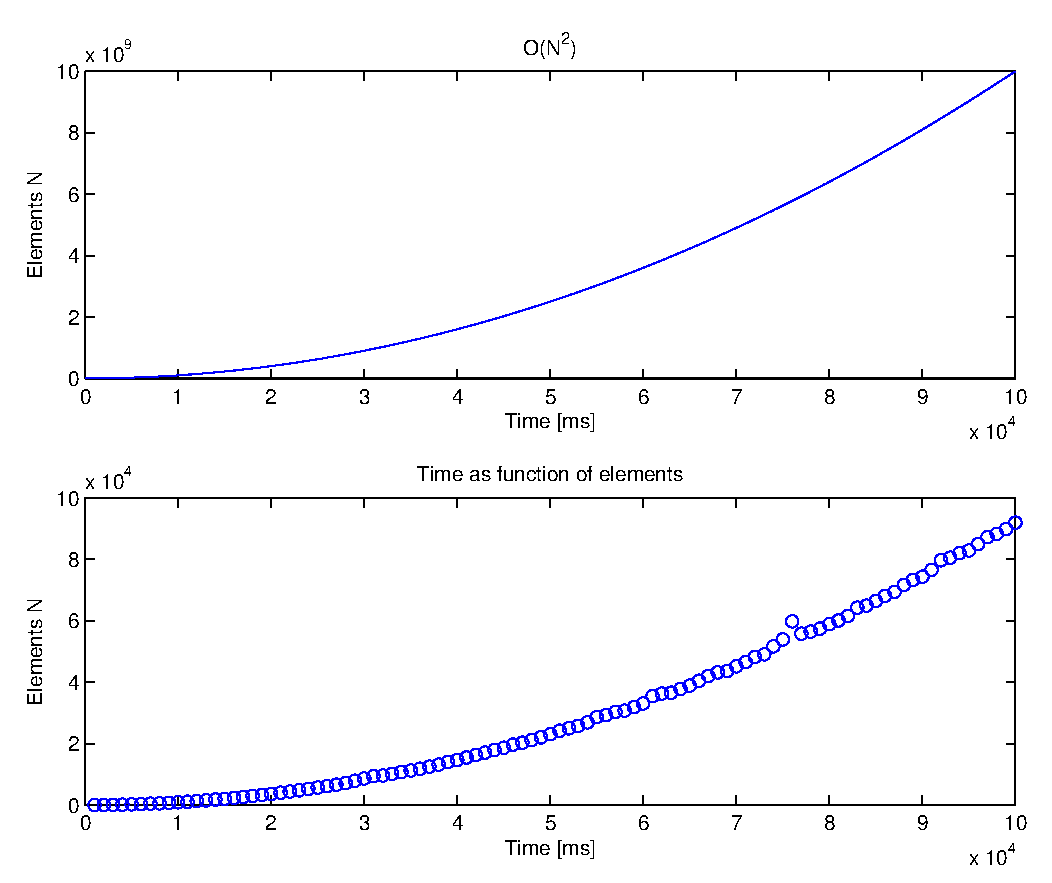
\includegraphics[width=1\textwidth]{./graphics/test1.eps}
\caption[tekst i indholdsfortegnelsen]{figurtekst}
\label{fig:}
\end{figure}
\newpage


\subsection{O(N Log(N)}
Figure \ref{fig:test2}


\todo[inline]{Description of the plot}
\begin{figure}[th!]
\centering
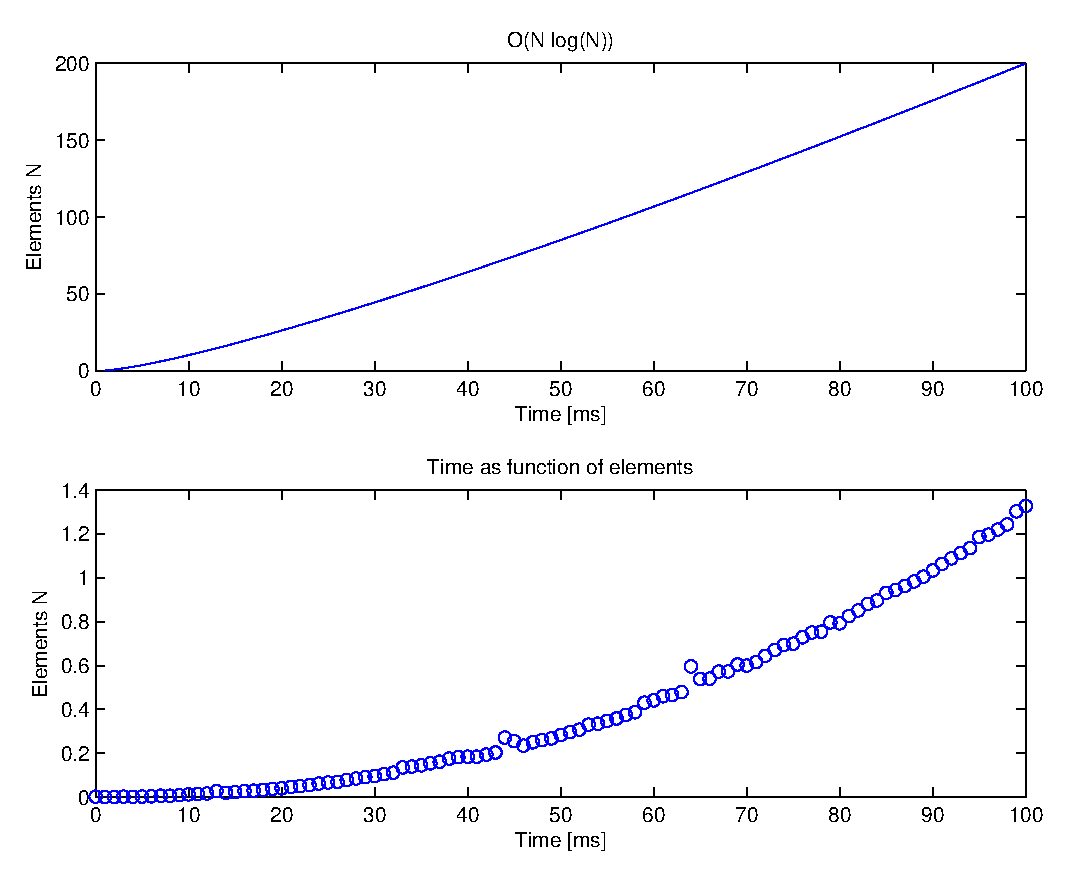
\includegraphics[width=1\textwidth]{./graphics/test2.eps}
\caption{Show plots of an ideal O(N log(N)) and data output from the algorithm.}
\label{fig:test2}
\end{figure}